\chapter{Methodology}
\label{chapter2}

<Everything that comes under the `Methodology' criterion in the mark scheme should be described in one, or possibly more than one, chapter(s).>

\section{Designing the simulator}
The current simulator is intentionally a \textbf{low-complexity tactical benchmark}, not yet a full race strategist. The learning agent does not control tyres, pit windows, fuel modes, or pace programmes. It currently learns one focused tactical problem: whether to hold position or attempt an overtake, with a selectable risk level, near configured overtaking zones.

To support later dissertation stages, the simulator contract is now externalised to \texttt{config.json}. Reward semantics, feedback features, experiment protocol, and stochasticity presets are all configured without changing agent code. This keeps algorithm comparisons methodological and reproducible.

\subsection{Modelling overtaking likelihood}
The track contains overtaking points where decisions can be made. FastF1 race telemetry is used to estimate where overtakes cluster and to assign zone difficulty. For this project scope, timing-loop based position updates are sufficient to produce a realistic relative difficulty map, even if they are not a full continuous on-track position model.

\begin{figure}
    \centering
    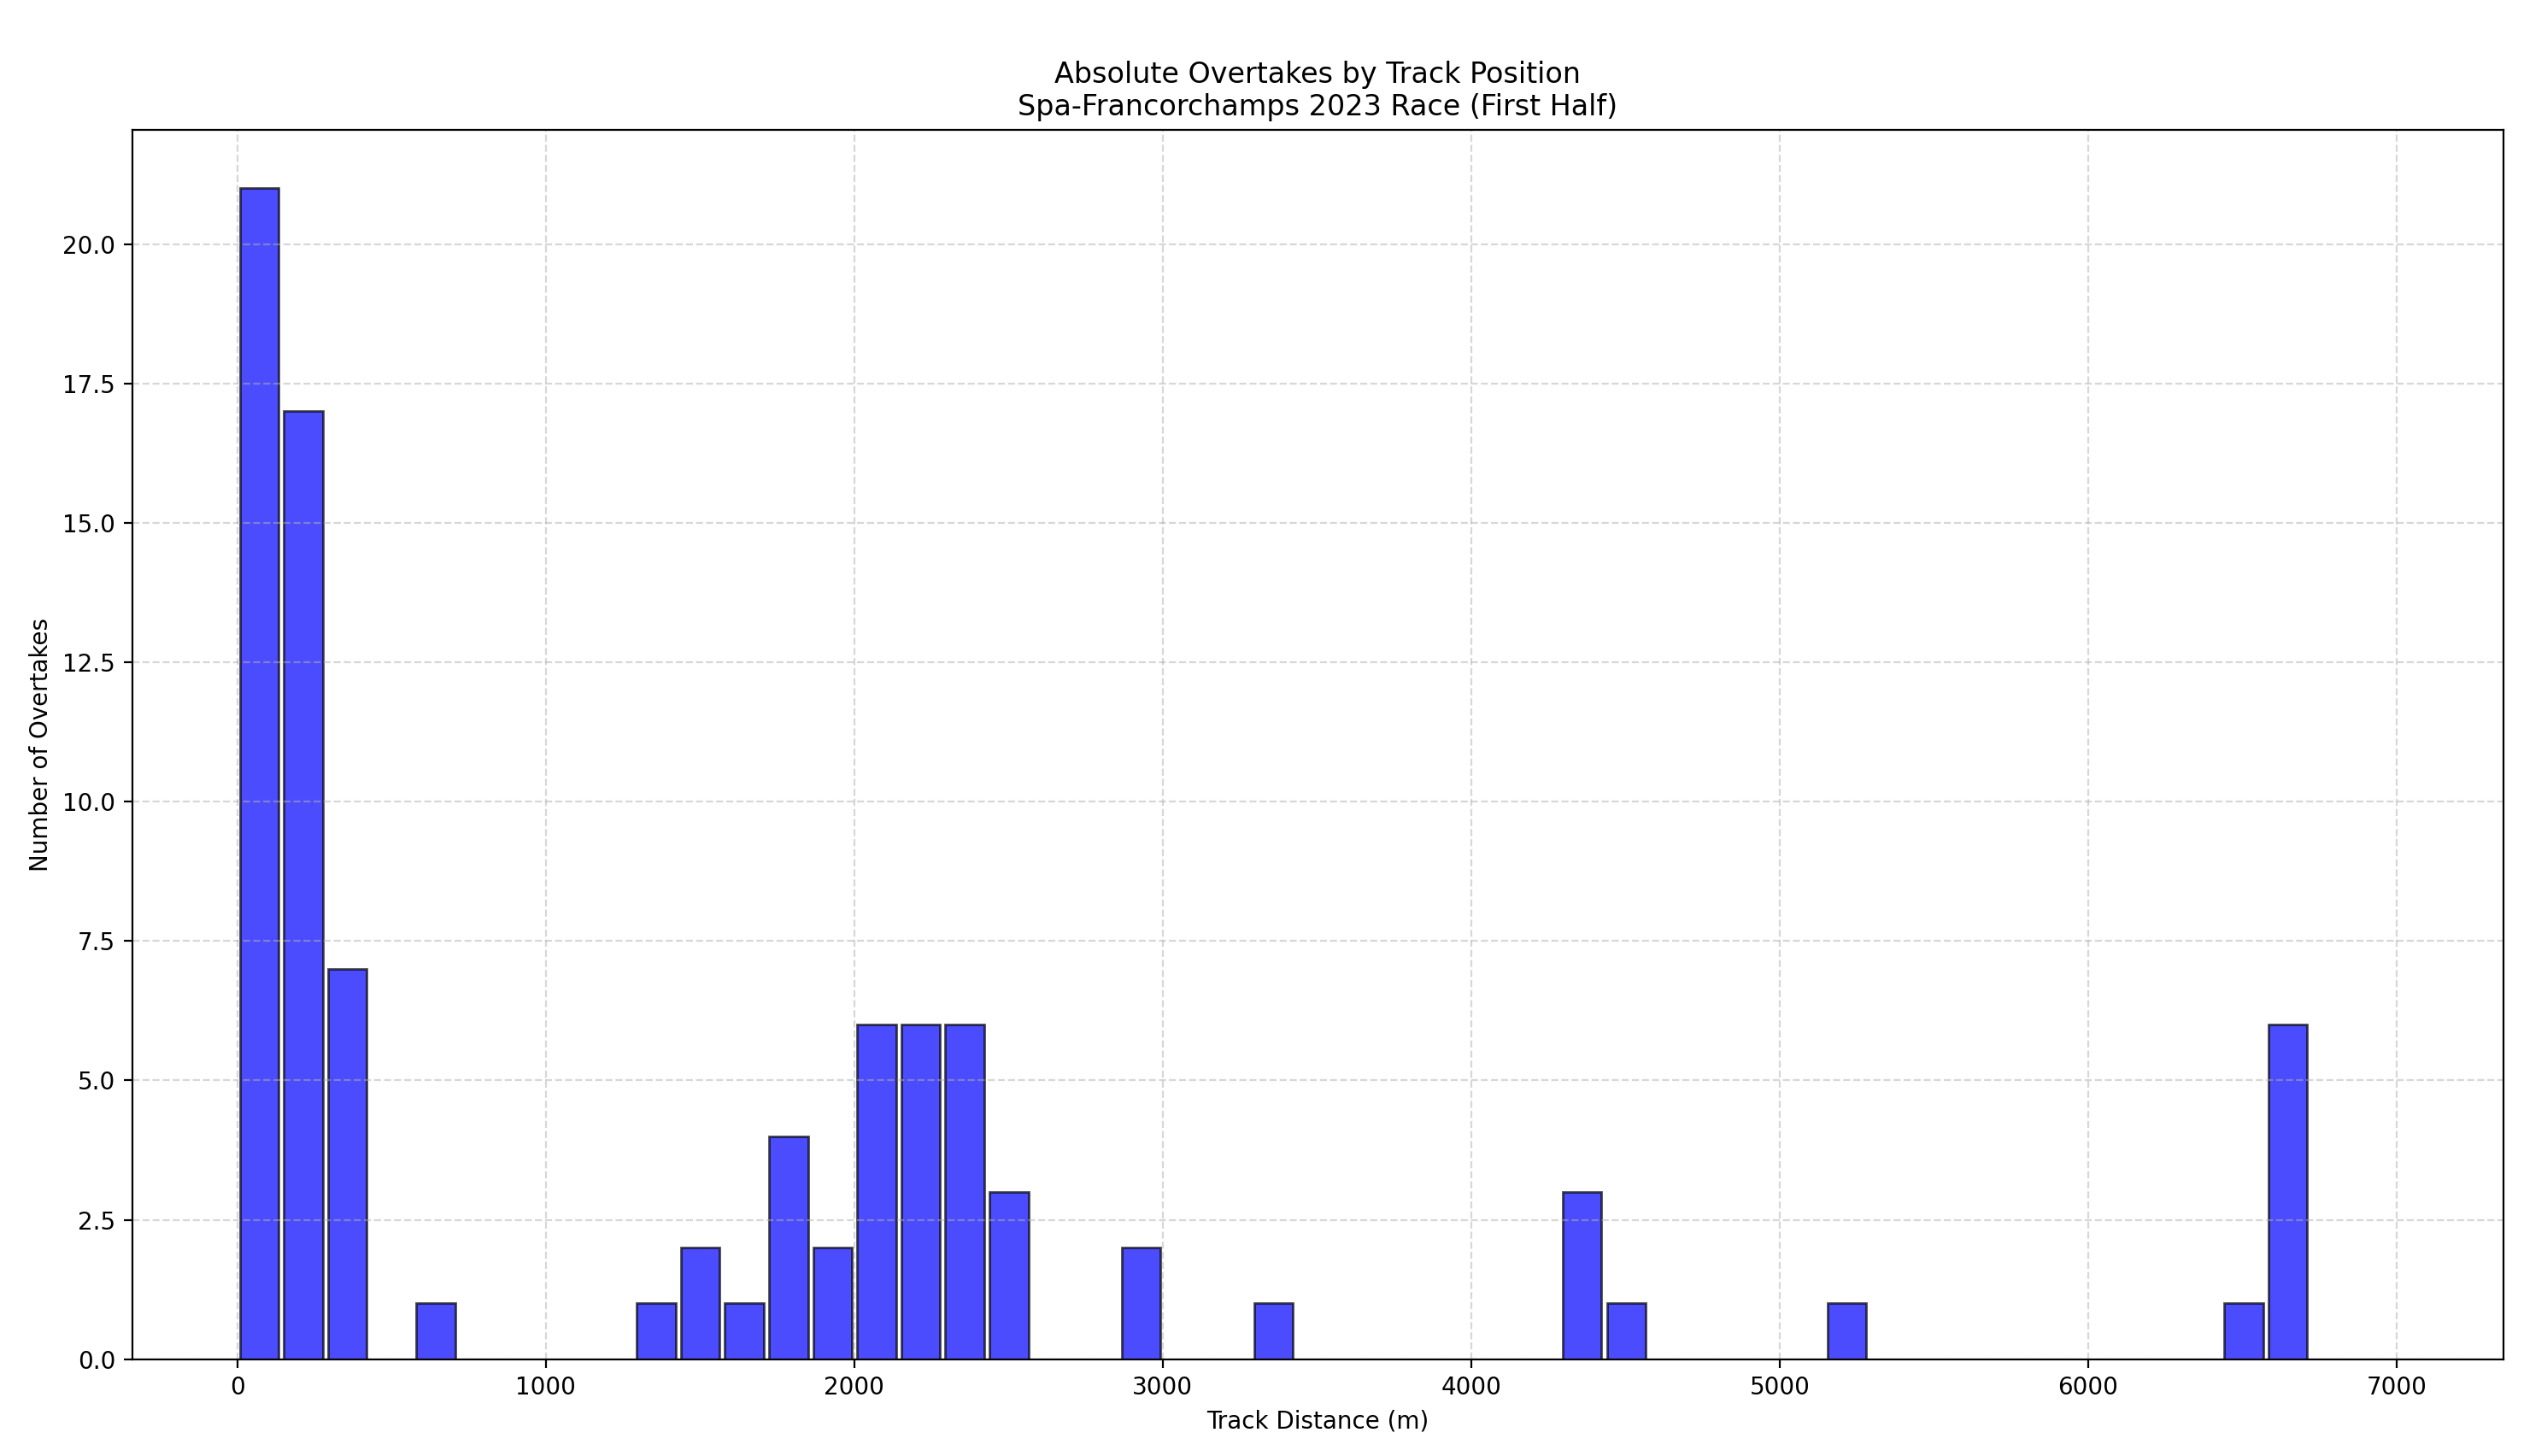
\includegraphics[width=0.5\linewidth]{NumberOfOvertakesSpa.png}
    \caption{Absolute overtakes based on distance on track}
    \label{fig:placeholder}
\end{figure}

\begin{figure}
    \centering
    
\includegraphics[width=0.5\linewidth]{overtakingMapping.png}
    \caption{Overtake density plotted over the circuit}
    \label{fig:placeholder}
\end{figure}

\subsection{Config-driven action and feedback contracts}
\subsubsection{Decision timing}
One decision is created when all of the following are true:
\begin{itemize}
    \item the driver is approaching an overtaking zone (within 0.2 km),
    \item there is a car ahead on track,
    \item the gap to that car is at most 0.1 km,
    \item the driver is not in the post-attempt cooldown window.
\end{itemize}
The decision is resolved when the driver reaches that zone.

\subsubsection{Action space}
Low complexity uses four discrete actions:
\begin{enumerate}
    \item hold position,
    \item attempt conservative overtake,
    \item attempt normal overtake,
    \item attempt aggressive overtake.
\end{enumerate}

\subsubsection{Feedback structure}
The observation contract is configured by \texttt{feedback.features\_by\_complexity}. In low complexity, the default profile includes:
\begin{enumerate}
    \item distance to next overtaking zone (normalised),
    \item gap to nearest car ahead (normalised),
    \item zone difficulty,
    \item binary indicator for whether a car ahead exists,
    \item current position (normalised),
    \item laps remaining (normalised).
\end{enumerate}
The active state dimension is derived from config, so all DQN-family algorithms consume the same observation contract in a given run.

\subsection{Finish-first reward contract}
Reward is defined with a fixed component schema across all tiers:
\[
R = R_{\text{outcome}} + R_{\text{persistent\_position}} + R_{\text{tactical}} + R_{\text{pace}} + R_{\text{tyre\_pit}} + R_{\text{penalty}}.
\]
In implementation, each component is normalised and weighted through \texttt{reward.weights}, \texttt{reward.normalization}, and \texttt{reward.component\_activation\_by\_complexity}.

For low complexity, only \texttt{outcome}, \texttt{persistent\_position}, \texttt{tactical}, and \texttt{penalty} are active; \texttt{pace} and \texttt{tyre\_pit} are forced to zero. This keeps one invariant reward meaning while allowing future complexity tiers to activate additional components without redefining the objective.

The objective hierarchy is finish-first:
\begin{itemize}
    \item \texttt{outcome} is terminal and dominant (start-to-finish position gain),
    \item \texttt{persistent\_position} provides dense shaping from position changes that survive decision resolution,
    \item \texttt{tactical} gives small local feedback for overtake outcomes with risk-scaled failure costs,
    \item \texttt{penalty} remains available for invalid/catastrophic behaviour.
\end{itemize}
Thus, overtaking is not the target itself; it is only valuable when it contributes to final race outcome.

\subsection{Complexity and stochasticity roadmap}
The methodology follows two independent expansion axes controlled in config:
\begin{enumerate}
    \item Train and validate on low complexity first.
    \item Increase complexity (low $\rightarrow$ medium $\rightarrow$ high) with the same reward schema.
    \item For each complexity level, evaluate across stochasticity presets (\texttt{s0} $\rightarrow$ \texttt{s1} $\rightarrow$ \texttt{s2}).
\end{enumerate}
Stochasticity levels are defined separately in \texttt{stochasticity.levels}, so robustness can be evaluated as performance drop under stress, not only raw score.

\section{Algorithm comparison protocol}
All comparison controls are externalised to \texttt{config.json}:
\begin{itemize}
    \item \texttt{protocol.seed\_sets}, \texttt{protocol.train\_runs}, and \texttt{protocol.eval\_runs} fix budgets and seeds,
    \item \texttt{protocol.comparison\_matrix.algorithms} fixes the DQN-family lineup,
    \item complexity and stochasticity schedules are controlled without editing agent internals.
\end{itemize}

Fairness is enforced by keeping the environment contract (state/reward/stochasticity) identical across vanilla, double, dueling, and rainbow-lite; only learning internals vary by algorithm.

\section{Evaluation and test protocol}
Testing is split into contract correctness, behavioural sanity, and benchmark fairness:
\begin{enumerate}
    \item \textbf{Config contract checks} before runs: validate reward/feedback/protocol/stochasticity keys, types, ranges, and compatibility.
    \item \textbf{Reward correctness checks} on each reward edit: verify total reward equals weighted normalised component sum and inactive low-tier components remain exactly zero.
    \item \textbf{Feedback correctness checks} on each feedback edit: verify state dimension matches configured active features and is identical across algorithms for the same scenario.
    \item \textbf{Behavioural sanity micro-scenarios}: safe hold, successful overtake, failed aggressive attempt, and persistent position gain; confirm finish-first dominance over overtake-count maximisation.
    \item \textbf{Fairness checks} on every benchmark matrix: identical seeds, train/eval budgets, complexity profile, and stochasticity level across algorithms.
\end{enumerate}

Recommended run cadence is:
\begin{itemize}
    \item smoke: 3 seeds,
    \item candidate: 5 seeds,
    \item benchmark/dissertation: 5 seeds with larger run budgets, fixed per comparison cell.
\end{itemize}
This provides statistical consistency while keeping computational cost manageable.

\section{Project management}
In order to maintain structure, and uphold good coding practices, the following standards were upheld.

\subsection{Software Development Lifecycle}
By adhering to the SDLC, we will do the necessary planning and research, then create an actionable plan for the scope and requirements of the project.

We also use sprints to keep track of objectives, and use working code as a measure of progress. 



\section{Software Architecture}
\subsection{Schematic diagram of project}
TBC

\subsection{Version control}
We use Git as a version control software.

\subsection{Good coding practice}
We assert that docstrings are used in any function, and when writing in Python, which is the primary language used in this project, we use snake case.

